\documentclass[a4paper, 12pt]{article}
\usepackage[margin=0.5in]{geometry}
\usepackage{graphicx}
\usepackage{caption}
\usepackage[section]{placeins}
\usepackage{fixltx2e}
\usepackage[page]{appendix}

\usepackage{amsmath}
\usepackage{cleveref}

%for code(MATLAB in particular)
\usepackage{listings}
\usepackage{color} %red, green, blue, yellow, cyan, magenta, black, white
\definecolor{mygreen}{RGB}{28,172,0} % color values Red, Green, Blue
\definecolor{mylilas}{RGB}{170,55,241}

% Default fixed font does not support bold face
\DeclareFixedFont{\ttb}{T1}{txtt}{bx}{n}{12} % for bold
\DeclareFixedFont{\ttm}{T1}{txtt}{m}{n}{12}  % for normal

% Custom colors
\usepackage{color}
\definecolor{deepblue}{rgb}{0,0,0.5}
\definecolor{deepred}{rgb}{0.6,0,0}
\definecolor{deepgreen}{rgb}{0,0.5,0}

\lstset{
    language=Matlab,%
    %basicstyle=\color{red},
    breaklines=true,%
    morekeywords={matlab2tikz},
    keywordstyle=\color{blue},%
    morekeywords=[2]{1}, keywordstyle=[2]{\color{black}},
    identifierstyle=\color{black},%
    stringstyle=\color{mylilas},
    commentstyle=\color{mygreen},%
    showstringspaces=false,%without this there will be a symbol in the places where there is a space
    numbers=left,%
    numberstyle={\tiny \color{black}},% size of the numbers
    numbersep=9pt, % this defines how far the numbers are from the text
    emph=[1]{for,end,break},emphstyle=[1]\color{red}, %some words to emphasise
    %emph=[2]{word1,word2}, emphstyle=[2]{style},
}


\graphicspath{{./pictures/}}

\title{ECEN321 - Lab 1}
\author{Joshua Benfell - 300433229}

\begin{document}
    \begin{figure}[!h]
        \centering
        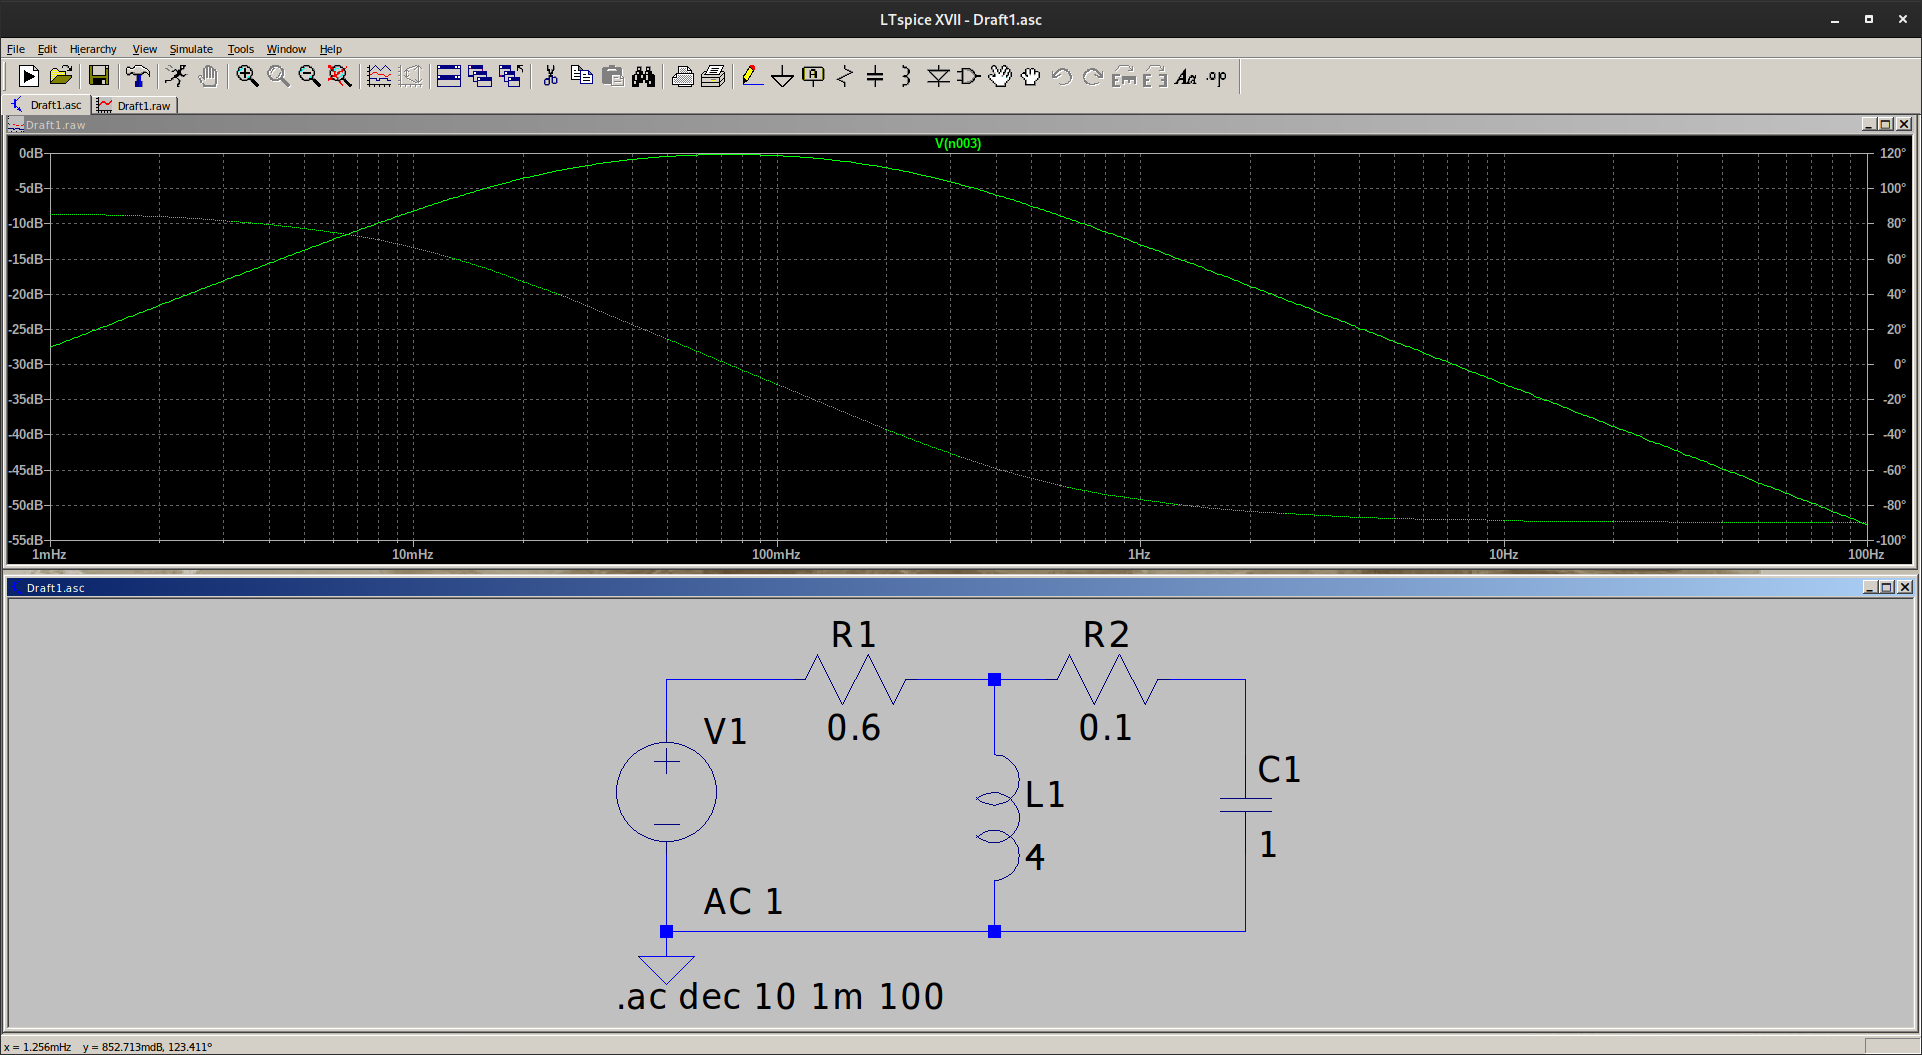
\includegraphics[width=\textwidth]{freqResponseSpice.png}
        \caption{Frequency response of the circuit in LTSpice}
        \label{fig:spiceF}
    \end{figure}
    \begin{figure}[!h]
        \centering
        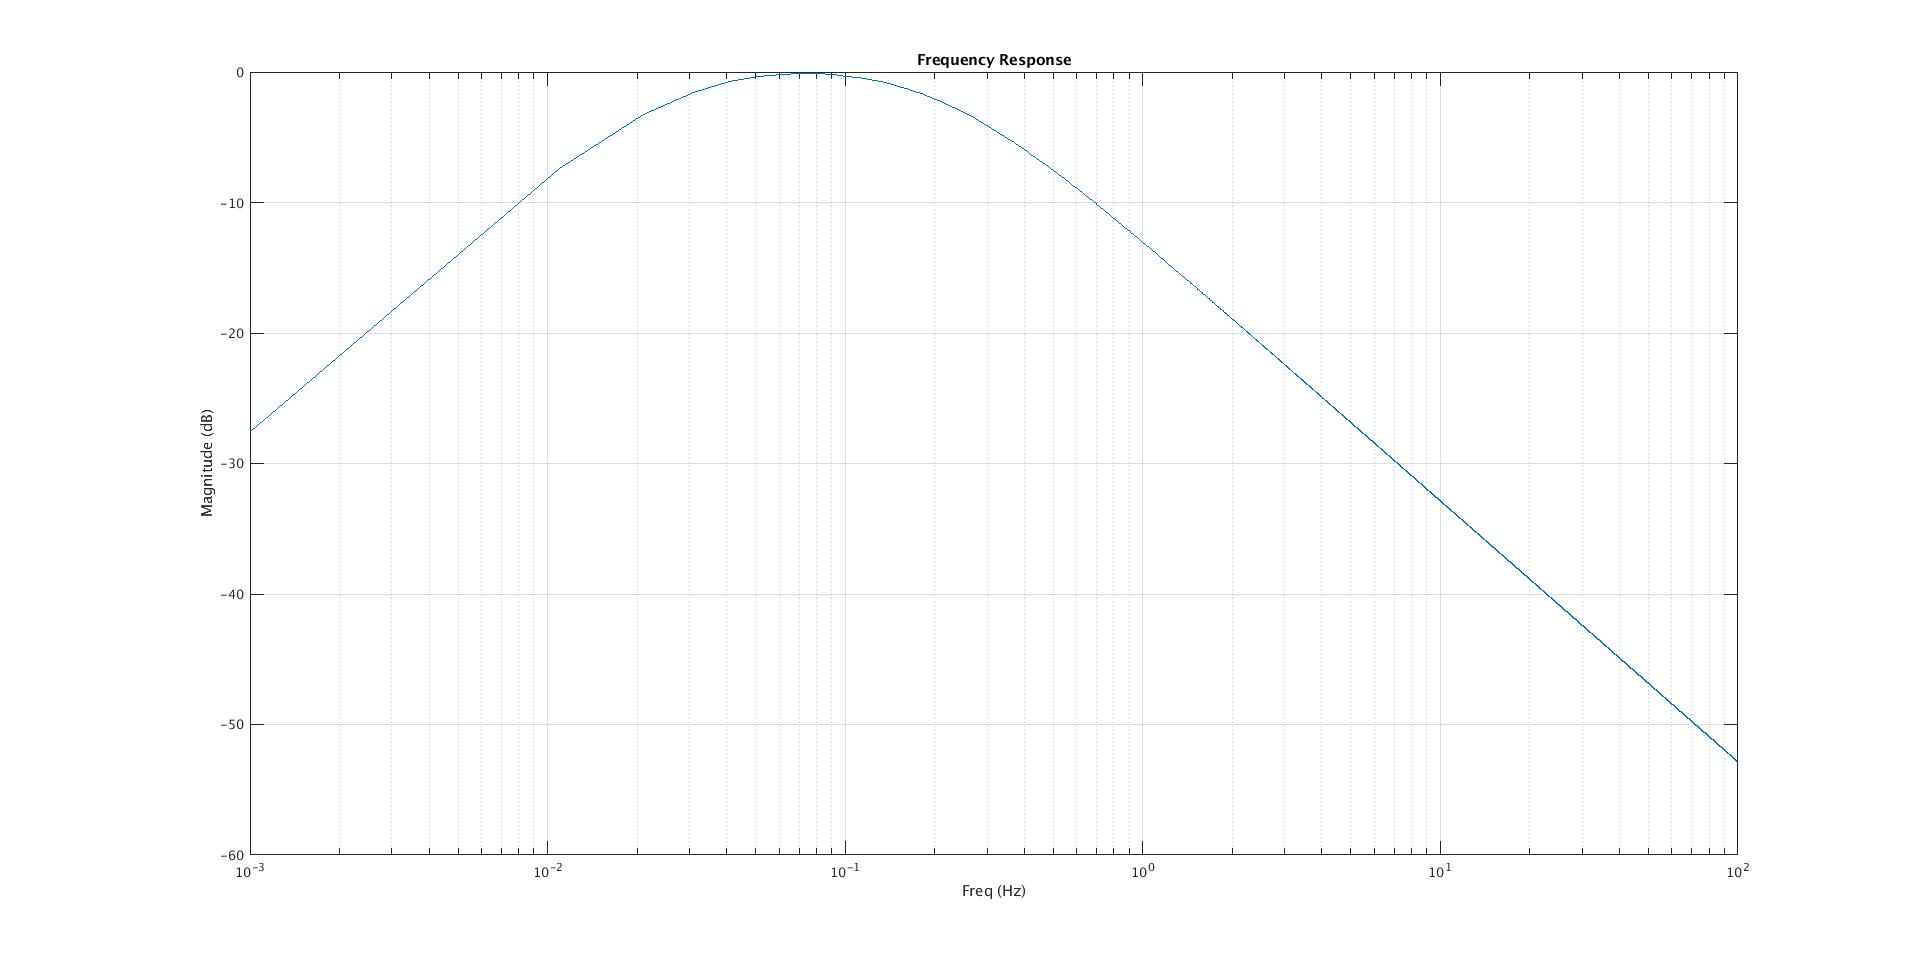
\includegraphics[width=\textwidth]{freqResponseMatlab.jpg}
        \caption{Frequency response of the transfer function in Matlab}
        \label{fig:matlabF}
    \end{figure}
    \begin{figure}[!h]
        \centering
        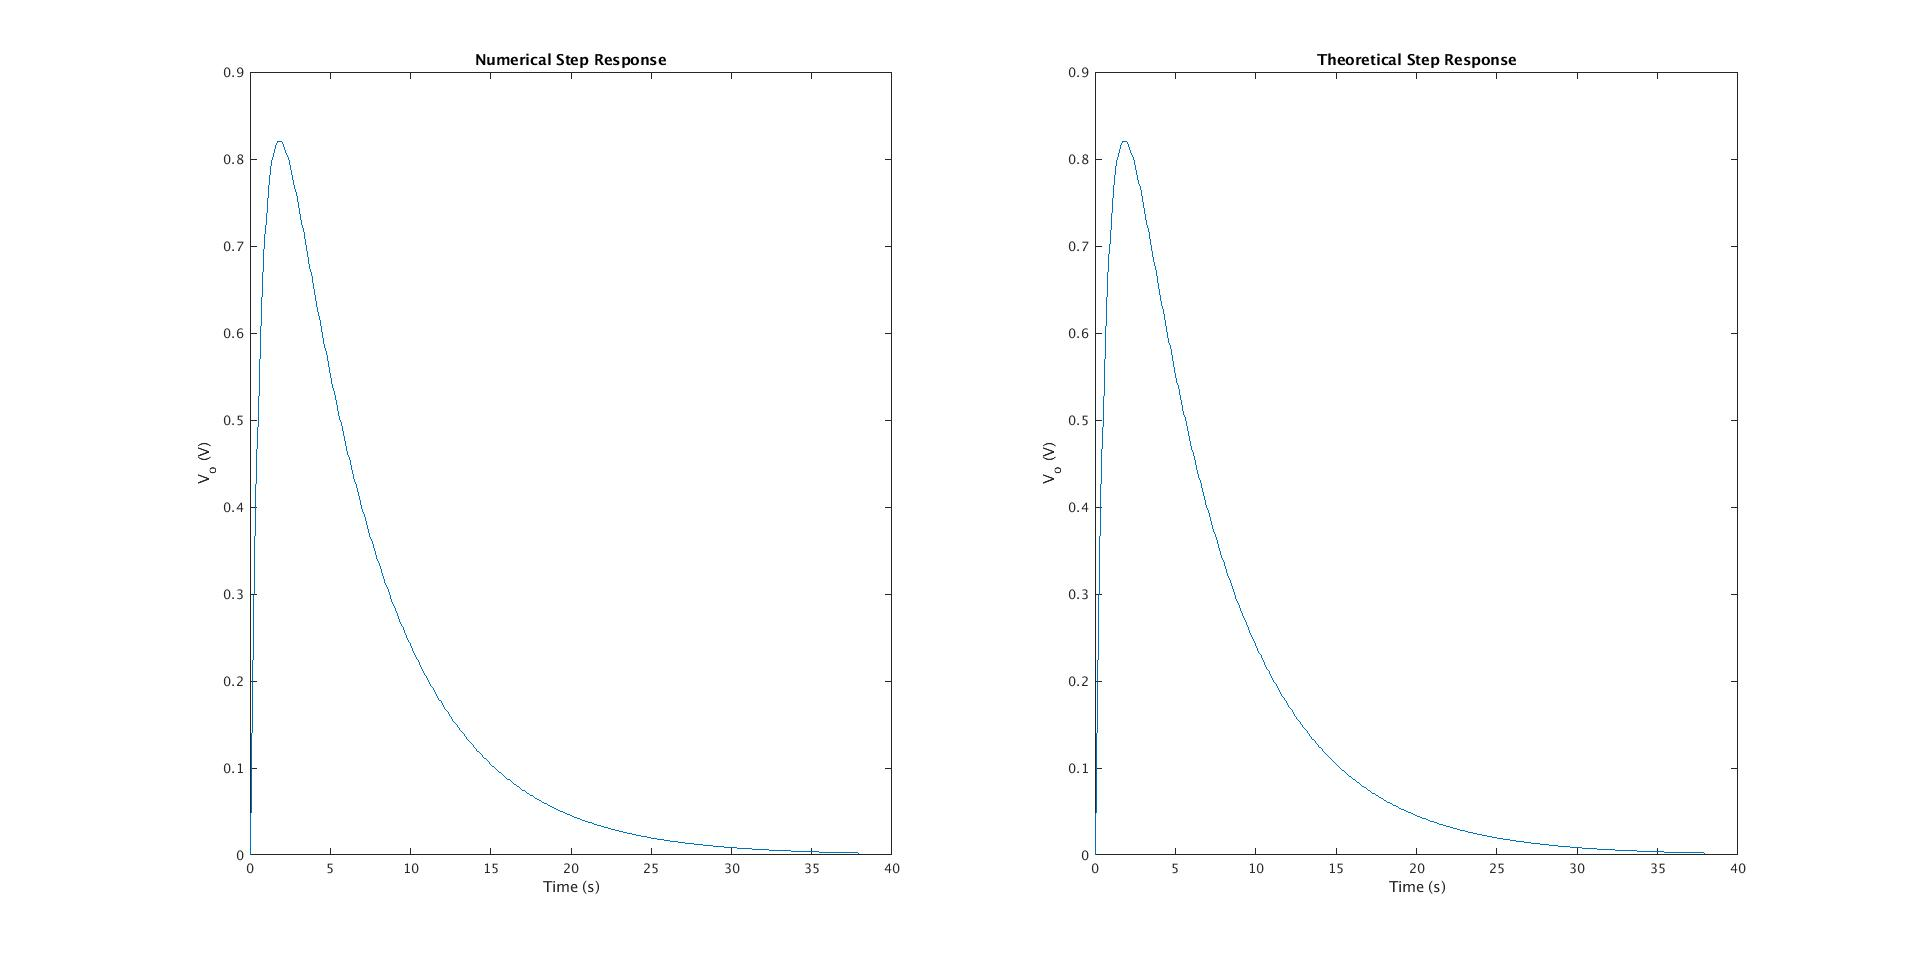
\includegraphics[width=\textwidth]{timeresponseplots.jpg}
        \caption{Time response to a step input in Matlab}
        \label{fig:matlabT}
    \end{figure}
    \pagebreak

    \Cref{fig:spiceF,fig:matlabF} show the frequency response of the circuit that was made in spice and the transfer function that was derived above. These plots are the same with gain in dB vs frequency in Hz and have the same intercepts and shape. This indicates a correct derivation.
    \par
    \Cref{fig:matlabT} contains both the numerical (left plot) and theoretical (right plot) time responses to a step input. The numerical one was found using the step function in matlab and the theoretical one was found by inverse laplace transform of the equation with a step response (shown above). As we can see though these are both pretty much identical indicating that the numerical methods are fairly accurate.
    \begin{appendices}
        \section{Matlab Code}\label{app:code}
            \lstinputlisting{ass1tf.m}
    \end{appendices}
\end{document}